\documentclass[12pt]{article}
\usepackage{graphicx}
\usepackage{enumitem}
\usepackage{amsmath}
\usepackage{gvv-book}
\usepackage{gvv}

\title{\textbf{4.10.8}}
\author{\textbf{EE25BTECH11008 - Anirudh M Abhilash}}
\date{October 2, 2025}

\begin{document}

\maketitle

\section*{Question}
Show that the area of the triangle formed by the lines $y=m_1x+c_1$, $y=m_2x+c_2$ and $x=0$ is
\[
\frac{(c_1-c_2)^2}{2\lvert m_1-m_2\rvert}.
\]

\section*{Solution}
Vertices:
\[
\vec{A} = \myvec{0\\c_1}, \quad \vec{B} = \myvec{0\\c_2}.
\]

Intersection of the two lines (RREF):
\begin{align}
\augvec{2}{1}{m_1 & -1 & -c_1 \\ m_2 & -1 & -c_2}
&\xrightarrow{R_2 \leftarrow R_2 - R_1}
\augvec{2}{1}{m_1 & -1 & -c_1 \\ m_2 - m_1 & 0 & -(c_2 - c_1)} \\
&\Rightarrow (m_2 - m_1)x = -(c_2 - c_1) \nonumber \\
&\Rightarrow x^* = \frac{c_2 - c_1}{m_1 - m_2}, \quad y^* = m_1 x^* + c_1.
\end{align}


Vectors:
\[
\vec{u} = \vec{AB} = \myvec{0\\c_2-c_1}, \quad
\vec{v} = \vec{AC} = \myvec{x^*\\y^*-c_1}.
\]

Observe that $y^* - c_1 = m_1 x^*$, hence
\[
\vec{v} = x^* \myvec{1\\m_1}.
\]

Compute norms and dot product:
\begin{align}
\|\vec{u}\|^2 &= (c_2-c_1)^2, \\
\|\vec{v}\|^2 &= x^{*2}(1+m_1^2), \\
\vec{u}\cdot \vec{v} &= (c_2-c_1)(m_1 x^*).
\end{align}

Using $\|\vec{u} \times \vec{v}\|^2 = \|\vec{u}\|^2 \|\vec{v}\|^2 - (\vec{u} \cdot \vec{v})^2$:
\begin{align}
\|\vec{u} \times \vec{v}\|^2 &= (c_2-c_1)^2 x^{*2}(1+m_1^2) - (c_2-c_1)^2 m_1^2 x^{*2} \\
&= (c_2-c_1)^2 x^{*2}.
\end{align}

Thus,
\begin{align}
\|\vec{u} \times \vec{v}\| &= |c_2-c_1|\,|x^*| = |c_2-c_1| \left| \frac{c_2-c_1}{m_1-m_2} \right| \\
&= \frac{(c_2-c_1)^2}{|m_1-m_2|}.
\end{align}

Area:
\begin{align}
\text{Area} &= \tfrac{1}{2} \|\vec{u} \times \vec{v}\| = \frac{(c_1-c_2)^2}{2|m_1-m_2|}.
\end{align}

\[
\boxed{\frac{(c_1-c_2)^2}{2|m_1-m_2|}}
\]

\begin{figure}[H]\centering
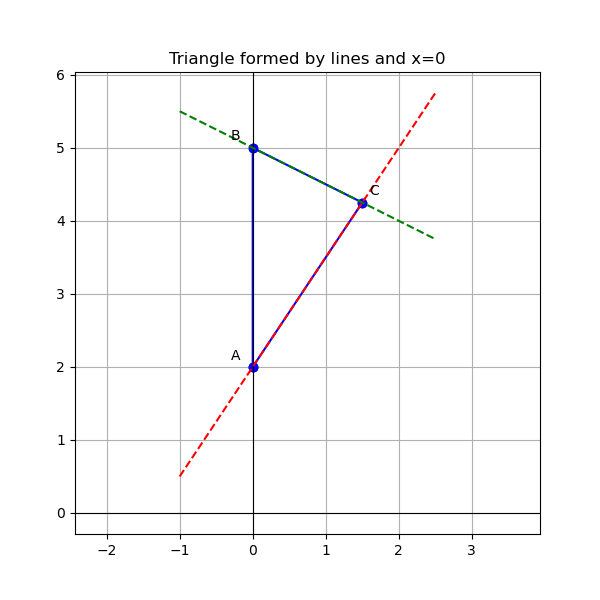
\includegraphics[width=1\columnwidth]{figs/plt.png}
\caption{Triangle formed by the lines and $x=0$}
\label{fig:plt}
\end{figure}

\end{document}
